\documentclass[10pt]{beamer}

\usepackage{enumerate}
\usepackage{tikz,tikz-cd,tikz-3dplot,pgfplots}
\usepackage{amsmath,amsthm,amssymb,amsfonts,amsthm}
\usepackage{mathrsfs}
\usepackage{bm,bbm}
\usepackage{braket}
\usepackage{slashed}
\usepackage{tensor}
\usepackage{indentfirst}
\usepackage{color}

\usetikzlibrary{decorations.markings,positioning,decorations.pathmorphing}
\allowdisplaybreaks
\pgfplotsset{width=10cm, compat=1.16}
\renewcommand\bra[1]{{\langle{#1}|}}
\renewcommand\ket[1]{{|{#1}\rangle}}
\renewcommand\bfdefault{b}

\DeclareMathOperator{\sech}{sech}
\DeclareMathOperator{\csch}{csch}
\DeclareMathOperator{\arcsec}{arcsec}
\DeclareMathOperator{\arccot}{arccot}
\DeclareMathOperator{\arccsc}{arccsc}
\DeclareMathOperator{\arccosh}{arccosh}
\DeclareMathOperator{\arcsinh}{arcsinh}
\DeclareMathOperator{\arctanh}{arctanh}
\DeclareMathOperator{\arcsech}{arcsech}
\DeclareMathOperator{\arccsch}{arccsch}
\DeclareMathOperator{\arccoth}{arccoth} 

\mode<presentation>
{
	\usetheme{Madrid}       % or try default, Darmstadt, Warsaw, ...
	\usecolortheme{default} % or try albatross, beaver, crane, ...
	\usefonttheme{serif}    % or try default, structurebold, ...
	\setbeamertemplate{navigation symbols}{}
	\setbeamertemplate{caption}[numbered]
}

\title{A light particle loop-effect on\\heavy particle propagator}
\author{S. Song}
\date{\today}

\begin{document}
	
	\begin{frame}
		\titlepage
	\end{frame}
	
	\begin{frame}{Outline}
		\tableofcontents
	\end{frame}
	
	\section{Model}
	\begin{frame}{Model}
		\begin{itemize}
			\item Lagrangian
			\begin{align*}
				\mathcal{L}=&\frac{1}{2}\partial_{\mu}\phi\partial^{\mu}\phi-\frac{m_{\phi}^{2}}{2}\phi^{2}-\frac{\Lambda_{3}}{6}\phi^{3}-\frac{\lambda_{4\phi}}{24}\phi^{4}\\
				&+\partial_{\mu}\chi^{\dagger}\partial^{\mu}\chi-m_{\chi}^{2}\chi^{\dagger}\chi-\frac{\lambda_{4\chi}}{4}(\chi^{\dagger}\chi)^{2}\\
				&+i\bar{\psi}_{1}\slashed{\partial}\psi_{1}+i\bar{\psi}_{2}\slashed{\partial}\psi_{2}-m_{\psi_{1}}\bar{\psi}_{1}\psi_{1}-m_{\psi_{2}}\bar{\psi}_{2}\psi_{2}\\
				&-T_{1}\phi\chi^{\dagger}\chi-\frac{\tau_{2}}{2}\phi^{2}\chi^{\dagger}\chi-Y_{1}\phi\bar{\psi}_{1}\psi_{1}-Y_{2}\phi\bar{\psi}_{2}\psi_{2}.
			\end{align*}
			(sign convention: $+,-,-,-$)
			
			\item No operators with higher than 4 mass dimension $\implies$ renormalisable $\implies$ No hard limit on parameters.
		\end{itemize}
	\end{frame}
	
	\begin{frame}
		\begin{itemize}
			\item Dimensionless parametrisation
			\begin{align*}
				\mathcal{L}_{\mathrm{scalar}}=&\frac{1}{2}\partial_{\mu}\phi\partial^{\mu}\phi-\frac{m_{\phi}^{2}}{2}\phi^{2}-\frac{\lambda_{3}m_{\phi}}{6}\phi^{3}-\frac{\lambda_{4\phi}}{24}\phi^{4}\\
				&+\partial_{\mu}\chi^{\dagger}\partial^{\mu}\chi-c^{2}m_{\phi}^{2}\chi^{\dagger}\chi-\frac{\lambda_{4\chi}}{4}(\chi^{\dagger}\chi)^{2}\\
				&-\tau_{1}m_{\phi}\phi\chi^{\dagger}\chi-\frac{\tau_{2}}{2}\phi^{2}\chi^{\dagger}\chi.
			\end{align*}
			
			\item To make perturbative expansion work:
			\[\lambda_{3},\lambda_{4\phi},\lambda_{4\chi},\tau_{2}\ll1,\quad\tau_{1}\ll c.\]
		\end{itemize}
	\end{frame}
	
	\section{Resonance Structure in One-Loop Order}
	\begin{frame}{Resonance Structure in One-Loop Order}
		One-loop diagrams
		\begin{center}
			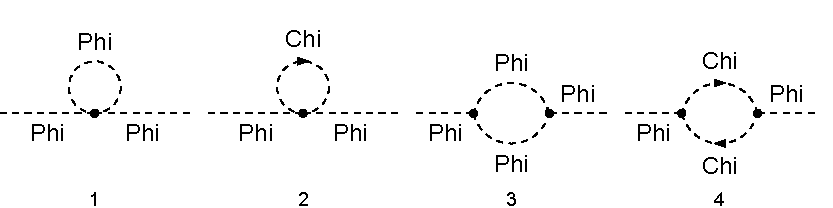
\includegraphics[width=10cm]{loopdiags.pdf}
		\end{center}
		Diagram 1 and 2 have no effects in one-loop order.
	\end{frame}
	
	\begin{frame}
		$|\tilde{\pmb{\Delta}}(s)|^{2}$ in terms of $s$:
		\begin{center}
			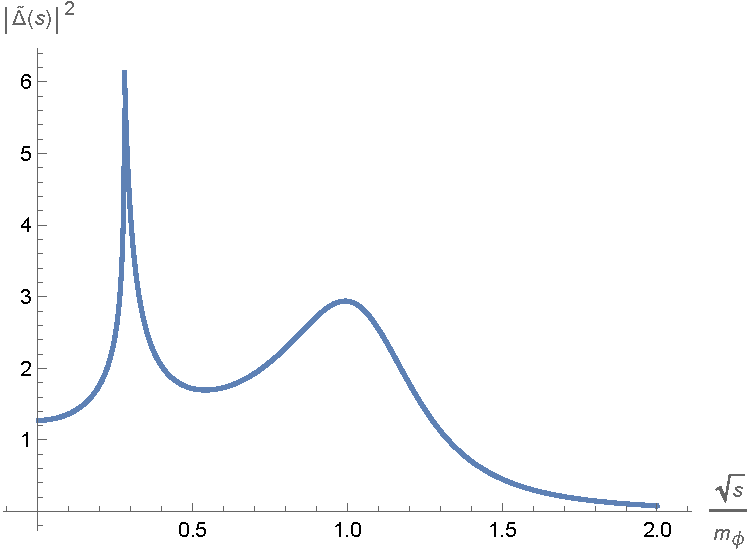
\includegraphics[width=7cm]{resonance1.pdf}
		\end{center}
		Parameters: $c=0.14$, $\lambda_{3}=0.15$, $\tau_{1}=0.13$.
		
		(Somewhat unrealistic in the sense that $\tau_{1}/c\approx 1$.)
	\end{frame}
	
	\begin{frame}
		More natural parameter settings:
		\begin{center}
			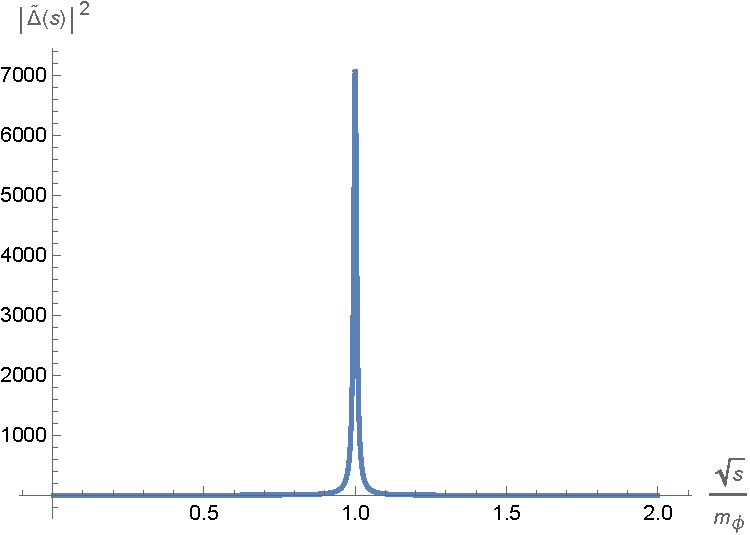
\includegraphics[width=7cm]{resonance2.pdf}
		\end{center}
		Parameters: $c=0.14$, $\lambda_{3}=0.15$, $\tau_{1}=0.02$.
		
		It appears to follow the Breit-Wigner distribution again.
		
		(The shape is highly dependent of $\tau_{1}$.)
	\end{frame}
	
	\begin{frame}
		Series expansion of $\Pi(s)$:
		\begin{align*}
			&\pi^{2}m_{\phi}^{2}\left[\frac{5\sqrt{3}\pi-27}{18}\lambda_{3}^2-3\tau_{1}^{2}-\frac{\tau_{1}^{2}(1-6c^{2})}{\sqrt{1-4c^{2}}}\log\left(\frac{1-\sqrt{1-4c^{2}}}{2c^{2}}-1\right)\right]\\
			&+\pi^{2}s\left[\frac{21-4\sqrt{3}\pi}{36}\lambda_{3}^{2}+\frac{\tau_{1}^{2}}{6}(6+\color{red}c^{-2}\color{black})-\frac{2c^{2}\tau_{1}^{2}}{\sqrt{1-4c^{2}}}\log\left(\frac{1-\sqrt{1-4c^{2}}}{2c^{2}}-1\right)\right]\\
			&+\frac{\pi^{2}s^{2}}{120m_{\phi}^{2}}\left(\lambda_{3}^{2}+\frac{2\tau_{1}^{2}}{\color{red}c^{4}\color{black}}\right)+\frac{\pi^{2}s^{3}}{840m_{\phi}^{4}}\left(\lambda_{3}^{2}+\frac{2\tau_{1}^{2}}{\color{red}c^{6}\color{black}}\right)+O(s^{4}).
		\end{align*}
		We have $c^{2}m_{\phi}^{2}=m_{\chi}^{2}$-suppression.
	\end{frame}
	
	\section{Alternative Model: Weak with Light Higgs}
	\begin{frame}{Alternative Model: Weak with Light Higgs}
		\begin{center}
			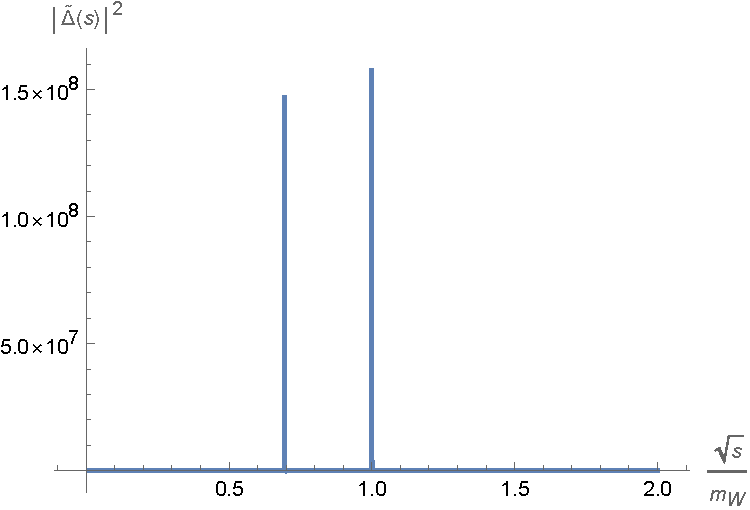
\includegraphics[width=7cm]{resonance3.pdf}
		\end{center}
		Parameters: $m_{H}/m_{W}=0.3$, $g_{W}=0.6$.
	\end{frame}
\end{document}